\chapter[バーの位置に基づく空中過程を含むブラキエーション動作]%
{バーの位置に基づく\\空中過程を含むブラキエーション動作}
\chaplabel{chapter4}
      \section{はじめに}
      

      空中過程を含むブラキエーション動作は,目標とするバーを把持することができなかった場合に落下してしまうという危険性がある.
      確実なバー把持のための条件には,バーとグリッパーの距離に加え,バーとの衝突を考慮することも望まれる.
      そこで,本研究では目標バーとロボットのグリッパー間の距離と,バー把持時のバーに対するグリッパーの相対速度に基づく評価関数を用いて
      振子過程で把持しているバーのリリース条件を最適化することを提案する.また,そのリリース条件を満たすように振幅調整を行い,空中過程を含むブラキエーション試行実験を行った.
      本章では,任意のバーの位置に基づくリリース条件最適化と,空中過程を含むブラキエーション実験の結果について述べる.

      \section{最適なバーリリース条件の導出}

      \subsection{最適化のための評価関数}
        \seclabel{J-define}
        
        バーを離すときの角度$\varphi$, 角速度$\dot{\varphi}$,ロボットの長さ$l_{\mathrm{r}}$の3つの値をバーリリース条件とする.
        安定したバー把持のための条件として,目標バーとグリッパーの距離が小さいこと,そしてバー把持時のバーに対するグリッパーの相対速度が小さいことが挙げられる.
        そこで,評価関数$J$を目標バー把持時の距離$J_{\mathrm{d}}$と相対速度$J_{\mathrm{r}}$
        を用いて\equref{J}とし,評価関数が最も小さくなる条件を求めた.
        ここで,$\alpha$は重み係数を表し,確実な把持のためにバーとグリッパーの距離に重みづけを行う.
        \begin{eqnarray}
          \equlabel{J}
          J(\varphi,\dot{\varphi},t,l_{\mathrm{r}})=\alpha{\times}J_{\mathrm{d}}+J_{\mathrm{r}}
        \end{eqnarray}
        評価関数が最小になるとき,目標とするバーとグリッパーの距離と相対速度がともに小さくなる.
        ゆえに,評価関数を最小にする角度$\varphi$, 角速度$\dot{\varphi}$,ロボットの長さ$l_{\mathrm{r}}$,
        リリース後のバー把持までの時間$t$を導出し,そのうち角度,角速度,ロボットの長さを最適なバーリリース条件とした.
        % また,バー把持までの時間はグリッパーを閉じるタイミングの決定に用いた.
        評価関数の最小化にはニュートン法と共役勾配法を組み合わせたNewton-CG法を用いた.

        \subsection{空中過程における目標バーとグリッパーの距離と相対速度}

          \figref{ReleaseFig2.eps}の状態でロボットが把持しているバーをリリースした場合,
          空中過程における目標バーとグリッパーの距離,相対速度を導出する.
          なお,空気抵抗は無視し,
          座標軸は左向きを$x$軸の正方向,上向きを$z$軸の正方向に設定し,
          ロボットが把持しているバーの座標を原点$(0,0)$,
          目標バーの座標を$(l_{\mathrm{bx}},l_{\mathrm{bz}})$とする.
          また,ロボットは姿勢$\varphi$とボディの全長$l_{\mathrm{r}}$の2変数を持つ.         
          ここで,バーリリース後の空中過程におけるロボットの長さ$l_{\mathrm{r}}$は
          バーリリース時から変えずに一定であるとすると, 
          ロボットの重心の軌道はバーリリース時の角度$\varphi$,角速度$\dot{\varphi}$による放物線軌道,
          手先の軌道はバーリリース時の角速度$\dot{\varphi}$による重心周りの一定速回転軌道となる.
          ゆえに,バーリリースから$t$秒後の目標バーとグリッパーとの距離$J_{\mathrm{d}}$,目標バーに対するグリッパーの相対速度$J_{\mathrm{r}}$は
          それぞれ\equref{Jd},\equref{Jr}で表される.
          ここで,$g$は重力加速度,$(x_{\mathrm{c}},z_{\mathrm{c}})$,$(\dot{x_{\mathrm{c}}},\dot{z_{\mathrm{c}}})$はロボットの重心の位置と速度,
          $(x_{\mathrm{e}},z_{\mathrm{e}})$,$(\dot{x_{\mathrm{e}}},\dot{z_{\mathrm{e}}})$はグリッパーの手先の位置と速度を表す.
          \begin{eqnarray}
            \equlabel{x-c}
            x_{\mathrm{c}}&=&\frac{1}{2}l_{\mathrm{r}}\dot{\varphi}\cos{(\varphi)}t+\frac{1}{2}l_{\mathrm{r}}\sin{(\varphi)}\\
            \equlabel{z-c}
            z_{\mathrm{c}}&=&\frac{1}{2}l_{\mathrm{r}}\dot{\varphi}\sin{(\varphi)}t-\frac{1}{2}gt^2-\frac{1}{2}l_{\mathrm{r}}\cos{(\varphi)}\\
            \equlabel{x-e}
            x_{\mathrm{e}}&=&x_{\mathrm{c}}+\frac{1}{2}l_{\mathrm{r}}\sin{(\varphi+\dot{\varphi}t)}\\
            \equlabel{z-e}
            z_{\mathrm{e}}&=&z_{\mathrm{c}}-\frac{1}{2}l_{\mathrm{r}}\cos{(\varphi+\dot{\varphi}t)}\\
            \equlabel{Jd}
              J_{\mathrm{d}}(\varphi,\dot{\varphi},t,l_{\mathrm{r}})
              &=&\sqrt{(l_{\mathrm{bx}}-x_{\mathrm{e}})^2+(l_{\mathrm{bz}}-z_{\mathrm{e}})^2}\\
            \equlabel{Jr}
            J_{\mathrm{r}}(\varphi,\dot{\varphi},t,l_{\mathrm{r}})
            &=&\sqrt{\dot{x_{\mathrm{e}}}^2+\dot{z_{\mathrm{e}}}^2}
          \end{eqnarray}  
        
          
        % \fig{barReleasefig.png}{width=0.6\hsize}{Schematic Diagram}
        \fig{ReleaseFig2.eps}{width=0.7\hsize}{Schematic Diagram in release}
        
        \subsection{評価関数を用いた最適なバーリリース条件の導出}
        実際の実験条件を\tabref{ExperimentConditions}に示す.
        ロボットの最大長0.74 mから5 cm離れた位置にある同じ高さのバーの条件である.
        また,その実験条件を基に求めた最適なバーリリース条件と評価値を\tabref{optimizedRelease}に示す.
        目標バーとグリッパーの距離の最小値$J_{\mathrm{d}}$が約1 mmであるため,バー把持が可能であると考えられる.
        

        \section{空中過程を含むブラキエーション実験}
        \subsection{目標振幅の導出}
        
          まず,\secref{J-define}において導出した最適なバーリリース条件になる目標振幅を決めた.
          \equref{Approximation Model},\equref{Approximation Angular velocity}を用いて,
          \equref{error}に示す評価関数$J_{\mathrm{e}}$を定義した.ここで,バーリリース条件の角度・角速度をそれぞれ
          $\varphi_{\mathrm{ref}}$,$\dot{\varphi}_{\mathrm{ref}}$とする.
          \begin{eqnarray}
            \equlabel{error}
            J_{\mathrm{e}}=\sqrt{(\varphi_{\mathrm{ref}}-\varphi(t))^2+(\dot{\varphi}_{\mathrm{ref}}-\dot{\varphi(t)})^2}
          \end{eqnarray}
          目標振幅からリリース条件到達までリンク長は一定であると仮定すると,
          伸縮を行わない単純な減衰振動となる.
          \secref{mokuhyou}で述べたように,単純な減衰振動において本研究では減衰率はロボット長に依存しないと考え,
          \equref{Approximation Model},\equref{Approximation Angular velocity}における振幅増加率を
          $\lambda=-0.04$とすることで減衰振動を表した.
          これを基に,半周期の間に評価関数$J_{\mathrm{e}}$を最小にする振幅$A$と時間$t$を求めた.
          評価関数の最小化にはNewton-CG法を用いた.
          これにより,求めた振幅$A$を目標振幅$A_{\mathrm{ref}}$とした.
          
          
          \subsection{リリース実験}

          \tabref{optimizedRelease}のリリース条件では目標振幅$A_{\mathrm{ref}} =$ 98 degと求まった.
          この目標振幅の検証のためのリリース実験を行った.
          \equref{Approximation Model},\equref{Approximation Angular velocity}を用いて
          振幅を$A_{\mathrm{ref}} =$ 98 degとした時の角度0 degからリリース条件角度$\varphi_{\mathrm{ref}} =$ 56 deg間の平均角速度を求めたところ300 deg/sであったため,
          リリース条件角度においてグリッパーがバーに引っかからない角度(50 deg)になるために要する時間$t_{\mathrm{gripper}}$を用いて,$300\times t_{\mathrm{gripper}}\approx$55 deg前にモータへ指令を行った.
          角度・角速度・リンク長の時間変化を\figref{release.eps},目標振幅到達後の実験の様子を\figref{releaseflow.eps}に示す.
          赤線はリリース条件角度に到達した時刻を示している.
          目標振幅到達時の計測振幅は99.1 degであり,導出した目標振幅98 degとの誤差は1.1 %となった.
          また,リリース時の角度・角速度はそれぞれ55.5 deg,254.1 deg/sであり,\tabref{optimizedRelease}に示したリリース条件との誤差はそれぞれ
          0.9 %,2.3 %であった.
          \begin{table}[tb]
            \begin{center}
              \caption{Experiment conditions}
              \tablabel{ExperimentConditions}
              \vspace{2mm}
              \begin{tabular}{c|c}
                \hline
                Variables & Values \\
                \hline
                $l_{\mathrm{bx}}$ [m] & 0.79 \\
                $l_{\mathrm{bz}}$ [m] & 0.00 \\
                $\alpha$ [-]& 20 \\
                $g$ $\mathrm{[m/s^2]}$ & 9.81 \\
                \hline
              \end{tabular}
            \end{center}
          \end{table}
          \begin{table}[tb]
            \begin{center}
              \caption{Optimized conditions values}
              \tablabel{optimizedRelease}
              \vspace{2mm}
              \begin{tabular}{c|c}
                \hline
                Variables & Values \\
                \hline
                $\varphi$ [deg] & 56 \\
                $\dot{\varphi}$ [deg/s] & 260 \\
                $l_{\mathrm{r}}$ [m] & 0.68 \\
                $t$ [s] & 0.261 \\
                $J$ [-] & 0.0144 \\
                $J_{\mathrm{d}}$ [m] & 0.00115 \\
                $J_{\mathrm{r}}$ [m/s] & 0.00292 \\
                \hline
              \end{tabular}
            \end{center}
          \end{table}
          \fig{release.eps}{width=0.6\hsize}{Release experiment data}
          \fig{releaseflow.eps}{width=0.65\hsize}{Release experiment flow}
          以上より,求めた振幅でのリリース条件の実現が可能であること確認することができた.
          しかし,リリース後に高さが足りないため目標のバーには到達できなかった.
          原因として,リリース時のグリッパーとバーの接触や,リリース後の空気抵抗,ケーブルの干渉などにより
          角速度が理論値よりも減少してしまったためであると考えた.
          そこでリリース条件の角度は変えずに,角速度のみ実験的にバーを把持できる高さに到達するように決定したところ約320 deg/sとなった.
          理論値と実際に必要な角速度との誤差を考慮して,\equref{error2}に示すように補正値$\dot{\varphi}_{\mathrm{revision}} =$60 deg/sを用いて評価関数$J_{\mathrm{e}}$を再定義した.
          これにより,目標振幅は119 degに変更された.
          \begin{eqnarray}
            \equlabel{error2}
            J_{\mathrm{e}}=\sqrt{(\varphi_{\mathrm{ref}}-\varphi(t))^2+(\dot{\varphi}_{\mathrm{ref}}+\dot{\varphi}_{\mathrm{revision}}-\dot{\varphi(t)})^2}
          \end{eqnarray}
          
          \subsection{ブラキエーション実験}
          変更後の目標振幅を用いて,空中過程を含むブラキエーション実験を行った.
          なお,バーリリース条件の角度は正であるため,求めた目標振幅は負の角度範囲における振幅である.
          目標バーの把持に成功した実験の計測データを図5.4,目標振幅到達後からの様子を\figref{Aerialflow.eps}(1)に示す.
          最適なバーリリース条件は,バー把持時のバーに対するグリッパーの相対速度が小さくなる条件であるため,
          実験においても衝撃が小さい把持であることが確認できた.また,目標振幅到達時の振幅は120.2 deg(誤差1.0 %),リリース時の角速度は318.1 deg/s(誤差0.6 %)であり,
          提案した振幅調整法により導出した目標振幅に到達し,最適なバーリリース条件を満たしたことが確認できた.
          なお,30回実験を行ったところ成功したのは2回であり成功率は約6.7 %であった.
          失敗した実験の計測データを\figref{AerialdataFailed.eps},目標振幅到達後からの様子を\figref{Aerialflow.eps}(2)に示す.
          目標振幅到達時の振幅は119.62 deg(誤差0.5 %)であるため把持失敗に影響していないとみられる.一方で,リリース時の角速度は275.5 deg/s(誤差14 %)であり,
          計測データを基にすると目標バーに届かない角速度である.しかし実際は\figref{Aerialflow.eps}(2-6)に示すように目標バーに届いているため,IMUへのノイズなどによる計測値のずれであると考えられる.
          
          さらに,バーに対するグリッパーの角度も考えられる.グリッパーの構造上,振子の回転軸方向に振動が発生しているため,
          目標バーに対して垂直にリリースされない場合がある.
          そのため、バー把持時のグリッパーの角度が影響して把持できなかったと考えられる.
          振子の回転軸方向に振動が発生しにくいグリッパー構造にすることで,より安定した把持が可能となり,成功率増加が期待できる.
          
          
          \begin{figure}[htbp]
            \begin{center}
            \figlabel{fig/Aerialdata}
            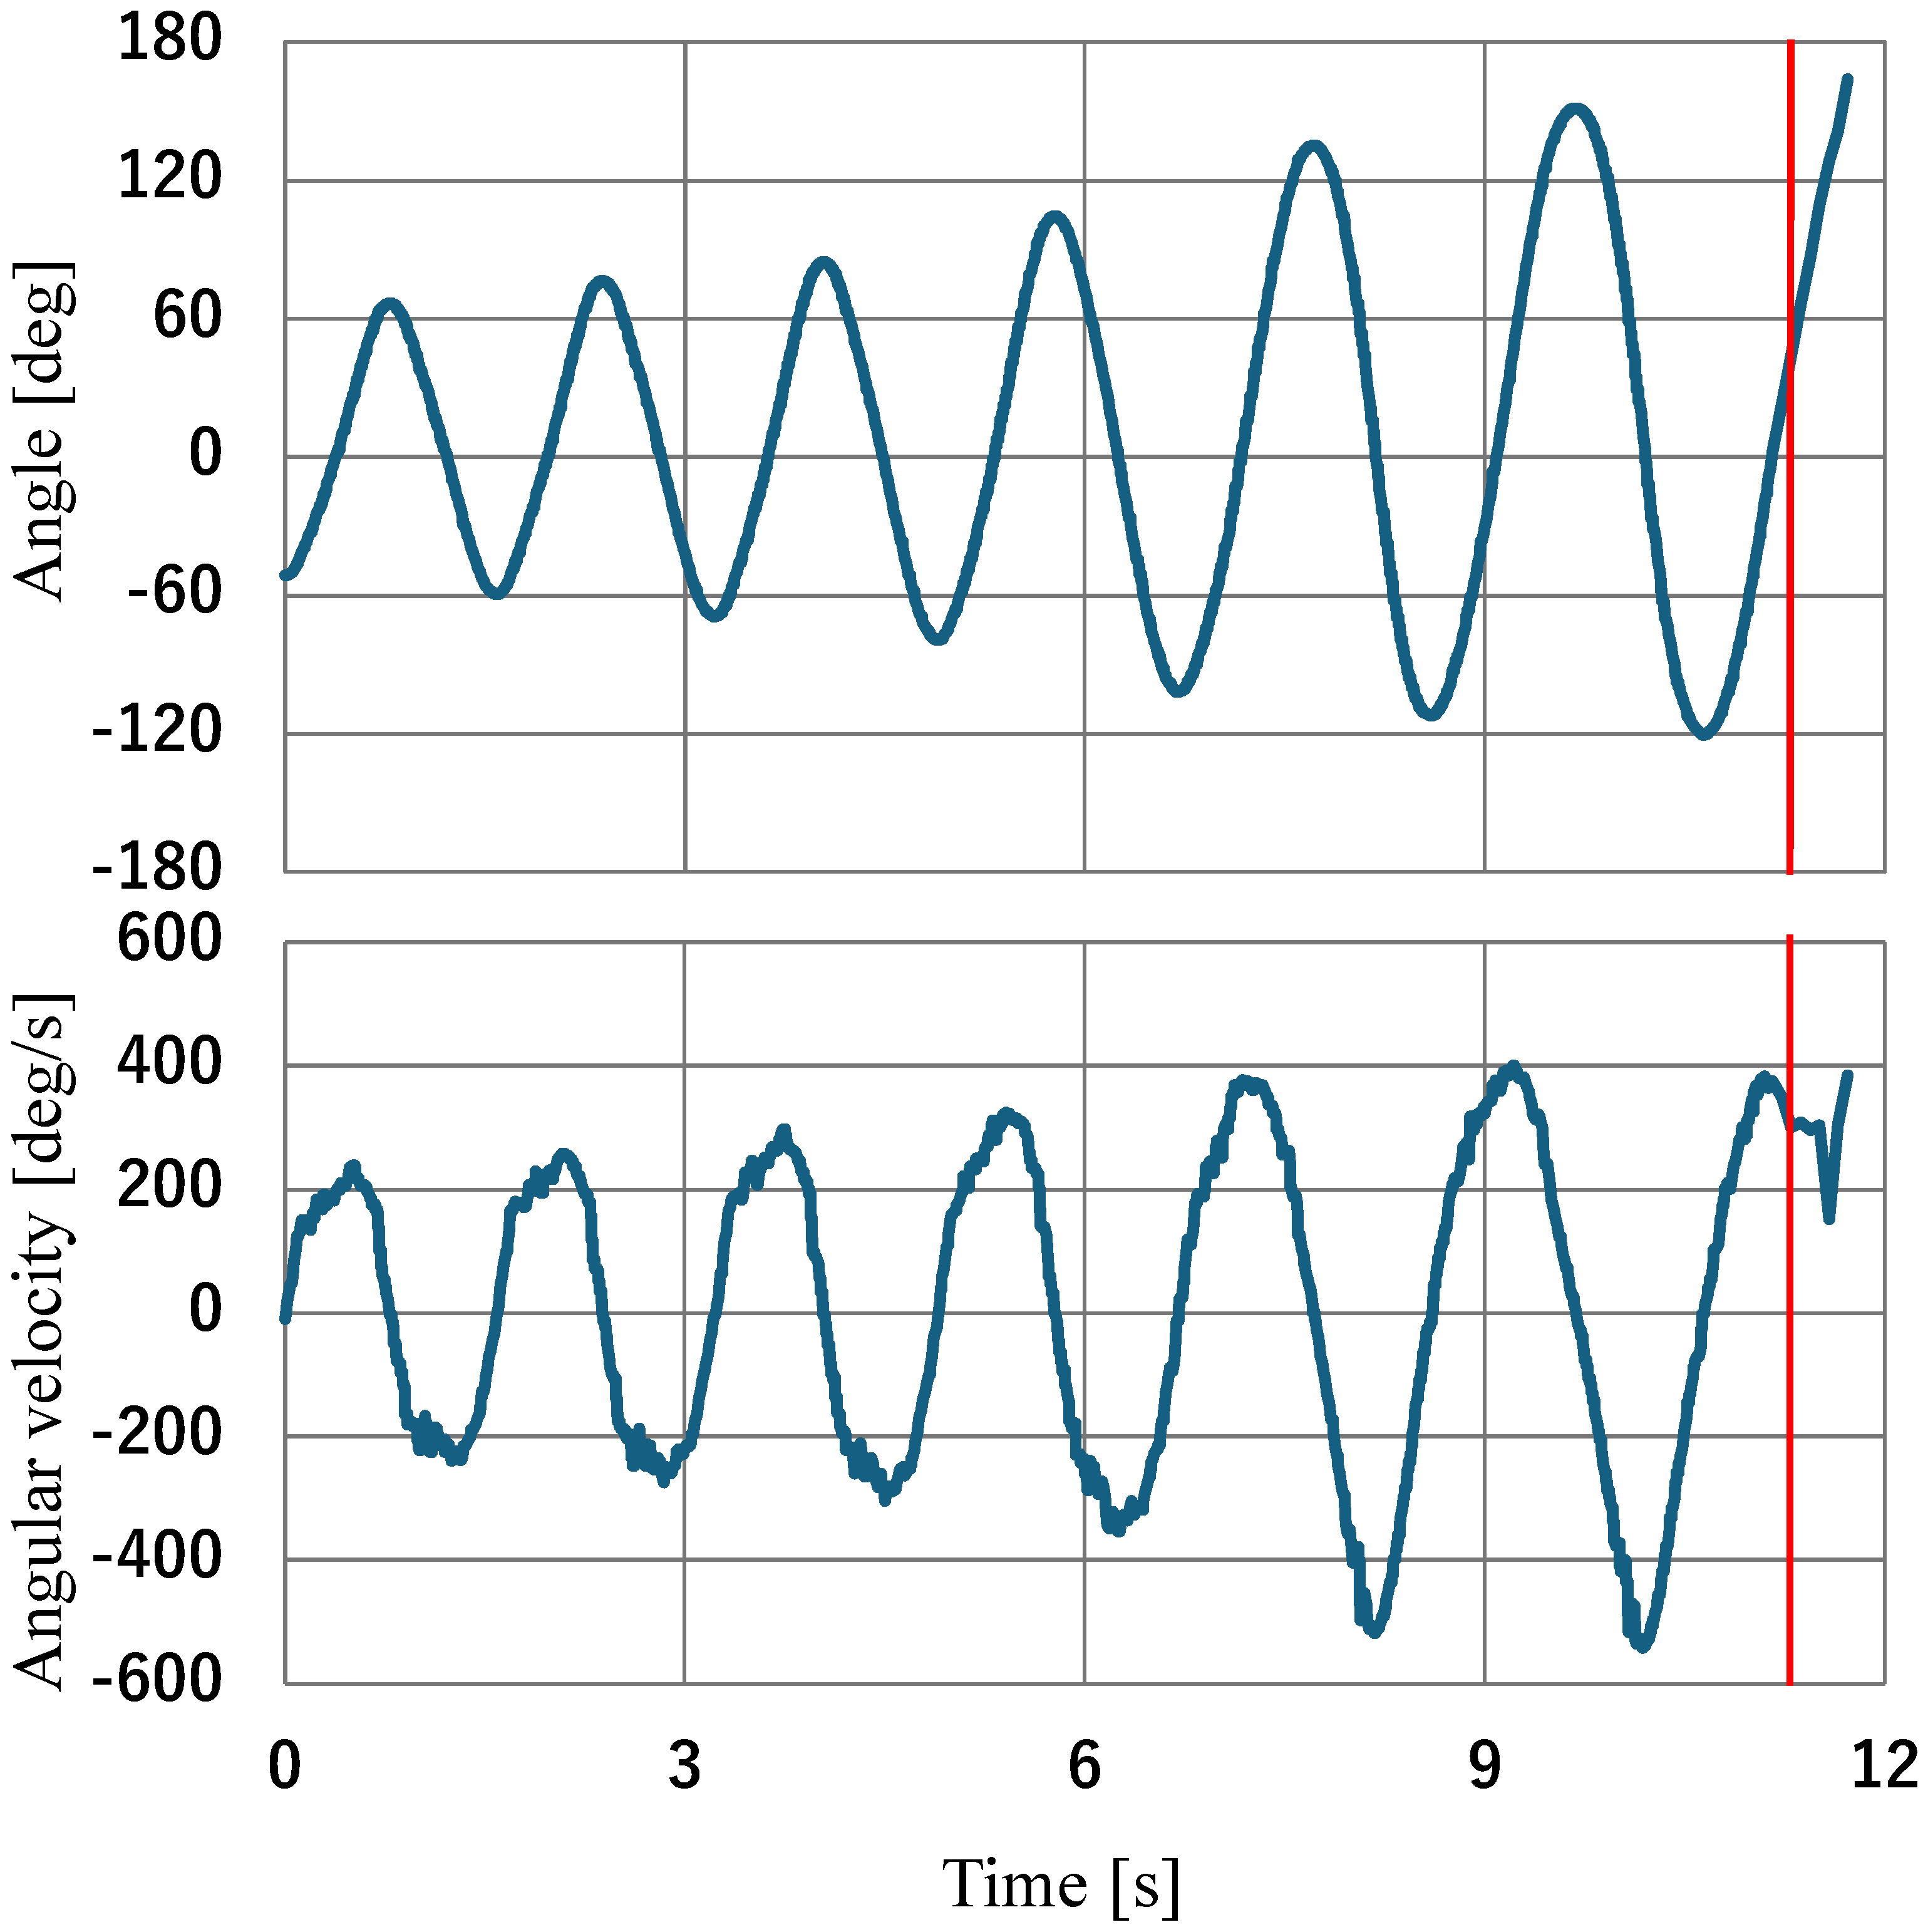
\includegraphics[width=100mm,height=100mm]{fig/Aerialdata.eps}
            \caption{Aerial Brachiation experiment data(Succeeded)}
            \end{center}
            \end{figure}
          \newpage
          % \fig{Aerialdata.eps}{width=0.7\hsize}{Aerial Brachiation experiment data(Succeeded)}
          \fig{AerialdataFailed.eps}{width=0.7\hsize}{Aerial Brachiation experiment data(Failed)}
          \fig{Aerialflow.eps}{width=0.7\hsize}{Aerial Brachiation experiment flow}
          




      
        % この最適なバーリリース条件が実用的かどうかを,次節で述べるリリース実験により確認した.
        
        % \subsection{実機実験}
        % 実験では,ロボットの長さが導出した条件で固定されるようにブラシレスモータを制御し,
        % 導出した角度・角速度になる初期振幅を実験的に求めた.
        % バーリリースの指令は,IMUで角度をリアルタイムに計測し,リリース条件の角度を満たした時にグリッパーが完全に開いた状態になるように
        % グリッパーのサーボモータの回転速度を考慮して設定した.
        % 同様にグリッパーを閉じるタイミングは,導出したバー把持までの時間を基にサーボモータの回転速度や空気抵抗などを考慮して
        % 実験的に決定した.
        
        % 実験の様子を\figref{ReleaseExperiment.eps}に示す.
        % 結果として,\secref{J-define}に基づいて導出した最適なバーリリース条件でのリリースによる
        % バー把持が可能であることを確認した.
        % また,バー把持時の衝撃が小さく,安定した把持であった.
        % これにより,評価関数に目標バーに対するグリッパーの手先の相対速度が小さくなる条件を含めることの有効性を確認した.
        % 一方,バーをリリースしてからバーを把持するまでの時間は0.24 sであり,\tabref{optimizedRelease}で示したバー把持までの時間と誤差が生じた.
        % その理由として,空中過程における空気抵抗や,バーリリース時のバーとの接触による摩擦などといった原因が考えられる.
        % より確実なバー把持のために,測距センサなどを用いてバーが近づいたらバーを自動的に把持するシステムなどが望まれる.
        
        % \fig{ReleaseExperiment.eps}{width=0.7\hsize}{Release Experiment}

